\documentclass{article}

\usepackage{siunitx} % Provides the \SI{}{} command for typesetting SI units
\usepackage{graphicx} % Required for the inclusion of images
\setlength\parindent{0pt} % Removes all indentation from paragraphs
\renewcommand{\labelenumi}{\alph{enumi}.} % Make numbering in the enumerate environment by letter rather than number (e.g. section 6)

%\usepackage{times} % Uncomment to use the Times New Roman font

%----------------------------------------------------------------------------------------
%	DOCUMENT INFORMATION
%----------------------------------------------------------------------------------------

\title{SFC} % Title
\author{Batman} % Author name
\date{\today} % Date for the report
\begin{document}
\maketitle % Insert the title, author and date

\begin{center}
\begin{tabular}{l r}
Date Performed: & December 31, 2013 \\ % Date the experiment was performed
Partners: & Robin \\ % Partner names
\end{tabular}
\end{center}

% If you wish to include an abstract, uncomment the lines below
% \begin{abstract}
% Abstract text
% \end{abstract}

%----------------------------------------------------------------------------------------
%	SECTION 1
%----------------------------------------------------------------------------------------

\section{Changes}

There is no significant update in SFC side.  
We only have three changes:
\begin{enumerate}
\item A new Cisco catalyst 2960G installation in SFC's NOC. 
\item A new NAT64 server based on OpenBSD-5.4-CURRENT.
\item Routing daemon updates to Quagga-0.99.22.4 in nara-gate router. 
\end{enumerate}

Because only a new NAT64 server has big significance in our operation, we will discuss in next paragraphs.  

\begin{figure}[h!]
\centering
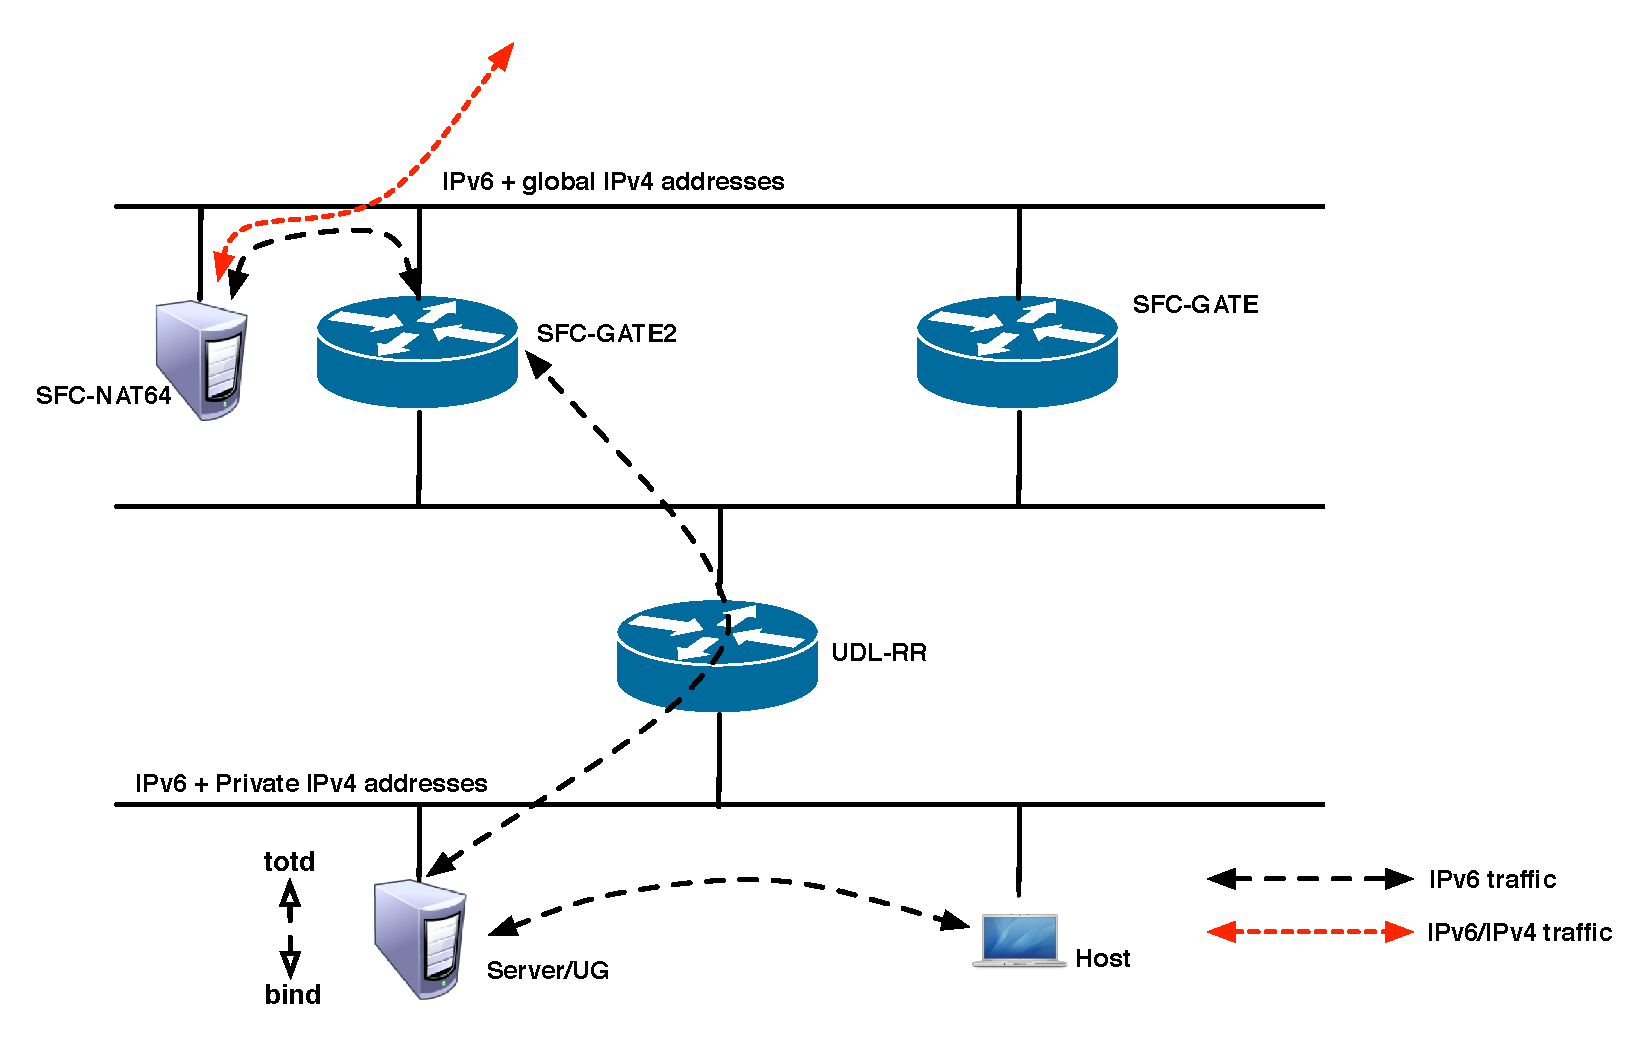
\includegraphics[width=1.\textwidth]{nat64}
\caption{Accessing IPv4 Internet via SFC-NAT64}
\end{figure}


\end{document}
